\documentclass[11pt]{article}

\usepackage{graphics} % or graphicx 
\usepackage{epstopdf}
\usepackage{multirow}
\usepackage{amsmath}
\usepackage{bbding}
\usepackage{pifont}
\usepackage{wasysym}
\usepackage{amssymb}
\usepackage{subcaption}
\usepackage{verbatim}


\setlength{\oddsidemargin}{0in}
\setlength{\textwidth}{6.5in}
\setlength{\topmargin}{-0.5in}
\setlength{\textheight}{8.75in}
\setlength{\parindent}{0pt}
\setlength{\parskip}{6pt}

\usepackage{fancyhdr}
\pagestyle{fancy}
\lhead{HW6} %----------------------------------------------------------- change
\rhead{Reza Shisheie}

\usepackage{epsfig,graphicx}

\usepackage{amsmath}

\usepackage{clrscode3e}

\begin{document}

\thispagestyle{plain}

\begin{center}
{\Large \bf CIS 606 \hfil Homework 6 \hfil Fall 2019} \\%--------------- change
\end{center}

\vskip 1in 

\centerline{\includegraphics[width=3in]{photo.jpg}}

\vskip 0.5in 


\begin{center}
\begin{tabular}{ll}
{\bf Name:}     & {\bf Reza Shisheie } \\ \\
{\bf Login ID:} & {\bf reshishe }   
\end{tabular}
\end{center}

\newpage

\begin{enumerate}

\itemsep 0.35in



\item Exercise 14.1-3 (page 344): Write a nonrecursive version of OS-SELECT .

	The recursive version of OS-Select is shown in the following:
		
	{\includegraphics[width=3in]{OS-Select.png}}
	
	On the non-recursive version, the function takes the root and the $i$the position and goes into a while loop.
	
	\begin{itemize}
     	\item In the while loop it calculates the current position of $x$, which is the left branch position plus 1 (self). $x$ is the root for the first run.  
     	
     	\item If the position matches the $i$the location, then this is the target. Therefore, $while$ loop breaks and position value is returned.
     
     	\item If $r$ as current position is larger than $i$, then target value is located in the left branch. Therefore, $x$ is updated to $x.left$ and while loop keeps executing the left branch for $i$th location. If $x.left$ is $null$ then such position does not exist. Therefore return -1. 
     	
     	\item If $r$ as current position is smaller than $i$, then target value is located in the right branch. Therefore, $x$ is updated to $x.right$ and while loop keeps executing the right branch for the remaining position which is $i-r$. If $x.right$ is $null$ then such position does not exist. Therefore return -1.
     	
     \end{itemize}
	
	
	 	
	
	\begin{codebox}
		\Procname{$\proc{OS-Select-NonRecursive}(x,i)$}
		
		\li \While $true$				
		\Do	
 		\li $r = x.left.size+1$
		\li \If $r=i$
		\li 	\Do
					return $x$
				\End
		
		\li \If $r<i$
				\Do	
		\li 		\If $x.left=\emptyset$
		\li 		\Do	
						return -1
					\End
				
		\li		$x = x.left$

		\li \ElseIf
		\li 	\Do	
		\li 		\If $x.right=\emptyset$
		\li 		\Do	
						return -1
					\End
					
		\li		$x \gets x.right$
		\li		$i \gets i-r$			
				\End
		\End
		
	\end{codebox}


\pagebreak


\item Exercise 14.3-6 (page 354) Show how to maintain a dynamic set $Q$ of numbers that supports the operation $\proc{Min-Gap}$ , which gives the magnitude of the difference of the two closest numbers in $Q$. For example, if $Q=\{1, 5, 9, 15, 18, 22\}$, then $\proc{Min-Gap}(Q)$ returns $18-15=3$, since 15 and 18 are the two closest numbers in $Q$. Make the operations $\proc{Insert}$, $\proc{Delete}$, $\proc{Search}$, and 
$\proc{Min-Gap}$ as efficient as possible, and analyze their running times.

	\textbf{MIN-GAP:} 

	The solution algorithm uses an RB-tree. A tuple is assigned to every element of set $Q$:
	
	\hspace{10mm} $x_i = \{key, min_{sub}, max_{sub}, gap\}$
	
	where, $key$ is the element value from $Q$, $min_{sub}$ is the minimum value in the sub branch, $max_{sub}$ is the maximum value in the sub branch, and $gap$ is the minimum gap between the following values:

	\begin{itemize}
		\item $x.key-x.left.max_{sub}$ : difference between current node and max node of left branch 
		\item $x.right.min_{sub}-x.key$ : difference between current node and min node of right branch
		\item $x.left.gap$ : minimum gap in the left branch
		\item $x.right.gap$ : minimum gap in the right branch
	\end{itemize}
    
	A visual look of the algorithm is shown in Figure.\ref{fig:prob-14-3-6}.
        
    \begin{figure}[h!]
		\centerline{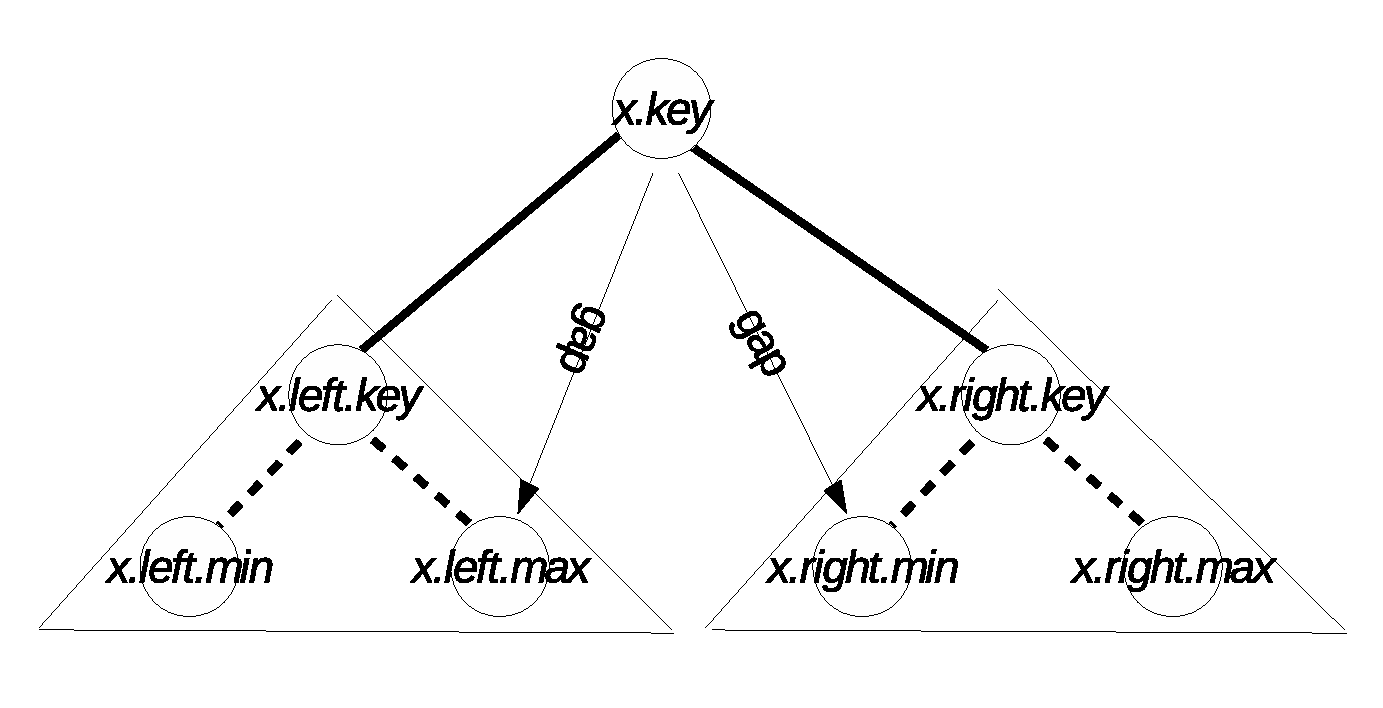
\includegraphics[width=4in]{prob-14-3-6.eps}}
		\caption{Algorithm branching}
		\label{fig:prob-14-3-6}
	\end{figure}

  	Before the $\proc{Min-Gap}(x)$ is executed, each tupe is initialized to:

	\hspace{10mm} $x_i= $
	\begin{math}
		\left\{
    		\begin{array}{l}
      			key = x_{value}\\
      			min_{sub} = x_{value}\\
      			max_{sub} = x_{value}\\
      			gap = +\infty
    		\end{array}
  		\right.
	\end{math}
	
	It is worth noting, since the first three parameters are initialized to $x_{value}$: 
	
	\begin{itemize}
		\item If the right branch does not have a subsequenct left branch ($x.right.left==\emptyset$), minimum value of the right branch ($x.right.min$) is the same as $x.right.key$
		\item Likewise if the left branch does not have a subsequenct right branch ($x.left.right==\emptyset$), maximum value of the left branch ($x.left.max$) is the same as $x.left.key$

	\end{itemize}
	
	The $\proc{Min-Gap}(x)$ algorithm only takes the $root$ and calucates minimum gap of each element and sub trees. Once its execution is over, $root.gap$ returns the minimum gap in the whole RB-tree.
	

	\begin{codebox}
		\Procname{$\proc{Min-Gap}(x)$}
		
		\li \Comment if there is no left or right child, this is the leaf$\rightarrow$return the gap parameters of $x$ which is $+\infty$ 

		\li \If $x.left=x.right=\emptyset$ 
		\li \Do 
				return 
			\End
		
		\li \Comment if there is no right child, $\rightarrow$ return $\proc{Min-Gap}(x.left)$ on the left branch 
		\li \ElseIf $x.right=\emptyset$ and $x.left \neq \emptyset$ 	
		\li \Do
				$\proc{Min-Gap}(x.left)$		 	

		\li \Comment if there is no left child, $\rightarrow$ return $\proc{Min-Gap}(x.right)$ on the right branch 
		\li \ElseIf $x.left=\emptyset$ and $x.right \neq \emptyset$ 	
		\li \Do
				$\proc{Min-Gap}(x.right)$

		\li \Comment if both children exist $\rightarrow$ return $\proc{Min-Gap}$ on the both right and left branches 
		\li \Else 	
		\li \Do
				$\proc{Min-Gap}(x.left)$
			\li $\proc{Min-Gap}(x.right)$
		\End
		
		\li \Comment Now min and max of current node has to be updated:
		\li \Comment if the min of the left branch<min of currect node $\rightarrow$ update min of current node
	 	\li \If $x.left.min_{sub} < x.min_{sub}$
		 	\li \Do 
			 	$ x.min_{sub}= x.left.min_{sub}$
			\End
		\li \Comment if the max of the right branch>max of currect node $\rightarrow$ update max of current node
		\li \If $x.right.max_{sub} > x.max_{sub}$
		 	\li \Do 
			 	$ x.max_{sub}= x.right.max_{sub}$
			\End


		\li $x.gap$ = min($x.key-x.left.max_{sub},$ 
		\li \hspace{21mm} $x.right.min_{sub}-x.key,$		 		
		\li \hspace{21mm} $gap.left,$
		\li \hspace{21mm} $gap.right$)	
		
		
		
	\end{codebox}

	
	
	
	
\pagebreak

	\textbf{INSERTION:} 

	For insertion two set of programs are recalled:
	\begin{itemize}
		\item $\proc{Insert}(x,v)$: This function takes node $v$ and recursively insert it into the RB-tree starting from $root$
		\begin{itemize}
			\item If the $v.key>x.key$: 
			\begin{itemize}
				\item If there exist a $x.right$ subtree, then node $v$ must be inserted into the right subtree $\rightarrow$	$\proc{Insert}(x.right,v)$
				\item Otherwise, this is the leaf $\rightarrow$ Insert node $v$ as new leaf to $x.right=v$ and return
			\end{itemize}
			\item If the $v.key\leq x.key$: 
			\begin{itemize}
				\item If there exist a $x.left$ subtree, then node $v$ must be inserted into the left subtree $\rightarrow$	$\proc{Insert}(x.left,v)$
				\item Otherwise, this is the leaf $\rightarrow$ Insert node $v$ as new leaf to $x.left=v$ and return
			\end{itemize}

		\end{itemize}

		\item $\proc{Min-Gap-Update-Node}(x)$: This function is a part of the $\proc{Min-Gap}(x)$ function, which updates $min_{sub}$, $max_{sub}$, and $gap$ of each node.  
	\end{itemize}


	
	\begin{codebox}
		\Procname{$\proc{Insert}(x,v)$}

	 	\li \If $v.key>\emptyset$
		 	\li \Do 
			 	return
			\End


	 	\li \If $v.key>x.key$
		 	\Do 
		 	\li \If $x.right\neq \emptyset$
			 	\li \Do 
				 	$\proc{Insert}(x.right,v)$
						 	
		 	\li \ElseIf $x.right= \emptyset$
			 	\li \Do 
				 	$x.right=v$
				 	\li return
				\End
			\End
		
	 	\li \If $v.key\leq x.key$
		 	\Do 
		 	\li \If $x.left\neq \emptyset$
			 	\li \Do 
				 	$\proc{Insert}(x.left,v)$
						 	
		 	\li \ElseIf $x.left= \emptyset$
			 	\li \Do 
				 	$x.left=v$
				 	\li return
				\End
			\End
			
		\li $\proc{Min-Gap-Update-Node}(x)$
		
	
		
	\end{codebox}

	
	\begin{codebox}
		\Procname{$\proc{Min-Gap-Update-Node}(x)$}
		
		\li \Comment if the min of the left branch<min of currect node $\rightarrow$ update min of current node
	 	\li \If $x.left.min_{sub} < x.min_{sub}$
		 	\li \Do 
			 	$ x.min_{sub}= x.left.min_{sub}$
			\End
		\li \Comment if the max of the right branch>max of currect node $\rightarrow$ update max of current node
		\li \If $x.right.max_{sub} > x.max_{sub}$
		 	\li \Do 
			 	$ x.max_{sub}= x.right.max_{sub}$
			\End


		\li $x.gap$ = min($x.key-x.left.max_{sub},$ 
		\li \hspace{21mm} $x.right.min_{sub}-x.key,$		 		
		\li \hspace{21mm} $gap.left,$
		\li \hspace{21mm} $gap.right$)	
		
			
	\end{codebox}


\pagebreak
	\textbf{DELETION:}
	
	DELETION, like INSERTION, follows the same rule of RB-tree deletion. Since all data is stored locally or in children, only an update on parents - from place of change - is needed. Thus, time complexity of INSERTION and DELETION are the height of RB-tree $O(\log{n})$. 

	\textbf{SEARCH:}
	
	The goal is to find the two nodes, which have the minimum gap. The same rule as for INSERTION and DELETION applies to SEARCH as well. Staring from root of RB-tree, trace the result of $\proc{Min-Gap}(x)$ value in the tree until both left and right braches yield larger $x.gap$ values. Calculating the minimum gap at this point, yields which two points yield the minimum gap. Therefore, time complexity of SEARCH is also $O(\log{n})$       

	









	
	
	
	
	
	





































   
\end{enumerate}

\end{document}

